% A simple template for Beamer presentations in LaTeX
% 
% To produce pdf run:
%   $ pdflatex beamer.tex 
%

\documentclass{beamer}
\usetheme{Singapore}

\hypersetup{colorlinks=true}

% Graphics examples
%\centerline{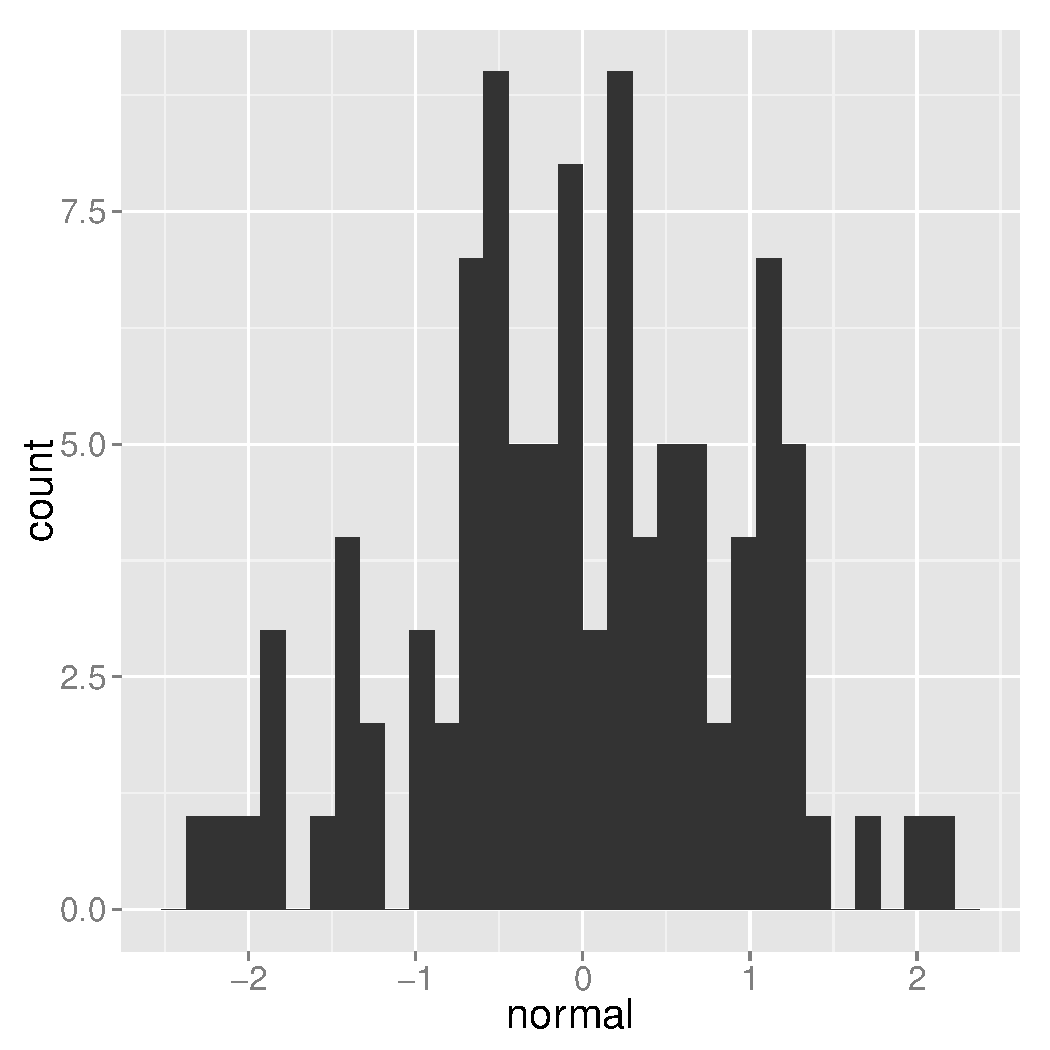
\includegraphics[height=2.5in]{figs/normal.pdf}}
%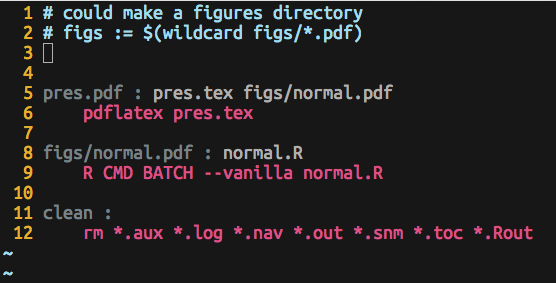
\includegraphics[width=4in]{figs/makefile.png}

%%%%%%%%%%%%%%%%%%%%%%%%%%%%%%%%%%%%%%%%%%%%%%%%%%%%%%%%%%%%

\begin{document}

\title[Python] % (optional, only for long titles)
{Distributions in Python}
\subtitle{random variables are easy with scipy.stats}
\author{Clark Fitzgerald - @clarkfitzg}
\institute{UC Davis - Statistics}
\date{24 November 2014} % (optional)
\subject{Statistics}

\frame{\titlepage}


%%%%%%%%%%%%%%%%%%%%%%%%%%%%%%%%%%%%%%%%%%%%%%%%%%%%%%%%%%%%
\begin{frame}


\frametitle{Topics}

\begin{itemize}

    \item Why I'm a bad programmer
    \item Introduction to scipy.stats (from Python!)
    \item Live Demo

\end{itemize}


\end{frame}
%%%%%%%%%%%%%%%%%%%%%%%%%%%%%%%%%%%%%%%%%%%%%%%%%%%%%%%%%%%%
\begin{frame}


    \frametitle{Why I'm a bad programmer}

    \begin{itemize}
        \item Error-prone
        \item Lazy
    \end{itemize}


\end{frame}
%%%%%%%%%%%%%%%%%%%%%%%%%%%%%%%%%%%%%%%%%%%%%%%%%%%%%%%%%%%%
\begin{frame}[fragile]


    \frametitle{The Binomial Distribution}

    \[
        X \sim \text{Binom} (10, 0.5)
\]
    
I'd like to know the probability mass function at 4.

    \emph{Is this code correct? incorrect?}

\begin{verbatim}
def f(n):
    'computes n!'
    return functools.reduce(operator.mul, range(n))

def binom(n, k):
    'computes n choose k'
    return f(n) / (f(k) * f(n - k))

def binom_pmf(n, p, k):
    'The probability mass function of Binom(n, p)'
    return binom(n, k) * p ** (n - k) * (1 - p) ** k
\end{verbatim}


\end{frame}
%%%%%%%%%%%%%%%%%%%%%%%%%%%%%%%%%%%%%%%%%%%%%%%%%%%%%%%%%%%%
\begin{frame}[fragile]

\emph{Is this code correct? incorrect?}

\textbf{Incorrect!}

\begin{verbatim}
binom_pmf(10, 0.5, 4)
\end{verbatim}


\end{frame}
%%%%%%%%%%%%%%%%%%%%%%%%%%%%%%%%%%%%%%%%%%%%%%%%%%%%%%%%%%%%
\begin{frame}


    \frametitle{Thoughts}

    \begin{itemize}
        \item algebra :(
        \item inefficient :(
        \item mistakes :(
        \item inconsistent :(
        \item maintenance :(
    \end{itemize}

\end{frame}
%%%%%%%%%%%%%%%%%%%%%%%%%%%%%%%%%%%%%%%%%%%%%%%%%%%%%%%%%%%%
\begin{frame}[fragile]

\[
        X \sim \text{Binom} (10, 0.5)
\]
    
I'd like to know the probability mass function at 4.

\emph{Is this code correct? incorrect?}

\begin{verbatim}
from scipy.stats import binom

X = binom(10, 0.5)
X.pmf(4)
\end{verbatim}

\textbf{Correct!}

I want to program the way I think, and just have it work perfectly.


\end{frame}
%%%%%%%%%%%%%%%%%%%%%%%%%%%%%%%%%%%%%%%%%%%%%%%%%%%%%%%%%%%%
\begin{frame}

    \frametitle{}

    With RV's we ask the same questions over and over.

    \begin{itemize}
        \item What's the mean?
        \item Given some data, what's the MLE for a parameter?
        \item Give me $n$ samples of some random variable $X$.
        \item What's the cdf of X with parameter $\beta$ evaluated at $k$?
    \end{itemize}

    That's why we had books of tables!

    But now we have computers.


\end{frame}
%%%%%%%%%%%%%%%%%%%%%%%%%%%%%%%%%%%%%%%%%%%%%%%%%%%%%%%%%%%%
\begin{frame}


\frametitle{Discrete distributions}

\textbf{13 discrete distributions}

bernoulli, 
binom, 
boltzmann, 
dlaplace, 
geom, 
hypergeom, 
logser, 
nbinom, 
planck, 
poisson, 
randint, 
skellam, 
zipf

\end{frame}

%%%%%%%%%%%%%%%%%%%%%%%%%%%%%%%%%%%%%%%%%%%%%%%%%%%%%%%%%%%%
\begin{frame}


\frametitle{Scipy Continuous Distributions}

\textbf{84 Continuous Distributions}

alpha, 
anglit, 
arcsine, 
beta, 
betaprime, 
bradford, 
burr, 
cauchy, 
chi, 
chi2, 
cosine, 
dgamma, 
dweibull, 
erlang, 
expon, 
exponweib, 
exponpow, 
f, 
fatiguelife, 
fisk, 
foldcauchy, 
foldnorm, 
frechet, 
variable, 
frechet, 
genlogistic, 
genpareto, 
genexpon, 
genextreme, 
gausshyper, 
gamma, 
gengamma, 
genhalflogistic, 
gilbrat, 
gompertz, 
gumbel, 
halfcauchy, 
halflogistic, 
halfnorm, 
hypsecant, 
invgamma, 
invgauss, 
invweibull, 
johnsonsb, 
johnsonsu, 
ksone, 
kstwobign, 
laplace, 
logistic, 
loggamma, 
loglaplace, 
lognorm, 
lomax, 
maxwell, 
mielke, 
nakagami, 
ncx2, 
ncf, 
nct, 
norm, 
pareto, 
pearson3, 
powerlaw, 
powerlognorm, 
powernorm, 
rdist, 
reciprocal, 
rayleigh, 
rice, 
recipinvgauss, 
semicircular, 
t, 
triang, 
truncexpon, 
truncnorm, 
tukeylambda, 
uniform, 
vonmises, 
wald, 
weibull, 
variable, 
weibull, 
wrapcauchy


\end{frame}
%%%%%%%%%%%%%%%%%%%%%%%%%%%%%%%%%%%%%%%%%%%%%%%%%%%%%%%%%%%%
\end{document}
